
\begin{figure}[H]
  {
    \setlength{\tabcolsep}{3.0pt}
    \setlength\cmidrulewidth{\heavyrulewidth} % Make cmidrule = 
    \begin{adjustbox}{height=5cm,center}
      \footnotesize
      \begin{tabular}{ll}

        \makecell[l]{
\icode{.BYTE \$00,\$01,\$02}\\
\icode{.BYTE \$00,\$FF,\$FE}
} & \makecell[l]{
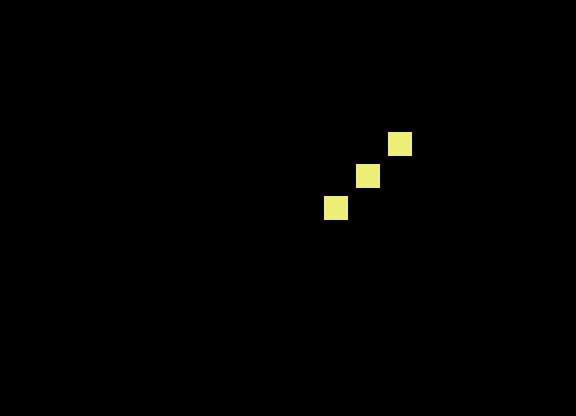
\includegraphics[width=1.3cm]{src/patterns/pixels/pixel_pattern14_0.png}%
} \\
        \midrule

        \makecell[l]{
\icode{.BYTE \$00,\$F6,\$F6}\\
\icode{.BYTE \$00,\$FC,\$FD}
} & \makecell[l]{
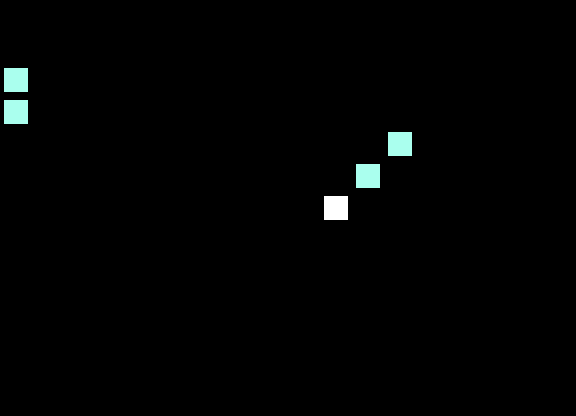
\includegraphics[width=1.3cm]{src/patterns/pixels/pixel_pattern14_1.png}%
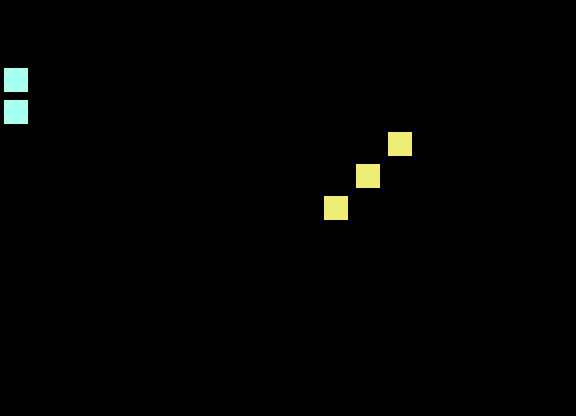
\includegraphics[width=1.3cm]{src/patterns/pixels/pixel_pattern14_2.png}%
} \\
        \midrule

        \makecell[l]{
\icode{.BYTE \$00,\$FB,\$FA,\$FB,\$FC}\\
\icode{.BYTE \$00,\$FA,\$FB,\$FC,\$FB}
} & \makecell[l]{

\includegraphics[width=1.3cm]{src/patterns/pixels/pixel_pattern14_3.png}%

\includegraphics[width=1.3cm]{src/patterns/pixels/pixel_pattern14_4.png}%
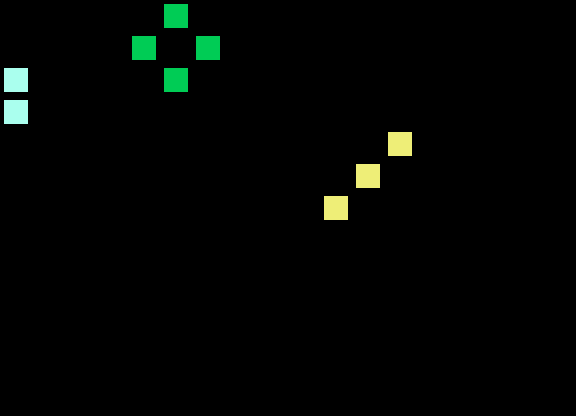
\includegraphics[width=1.3cm]{src/patterns/pixels/pixel_pattern14_5.png}%
} \\
        \midrule

        \makecell[l]{
\icode{.BYTE \$00,\$FD,\$FD,\$FE,\$FE}\\
\icode{.BYTE \$00,\$05,\$06,\$06,\$05}
} & \makecell[l]{
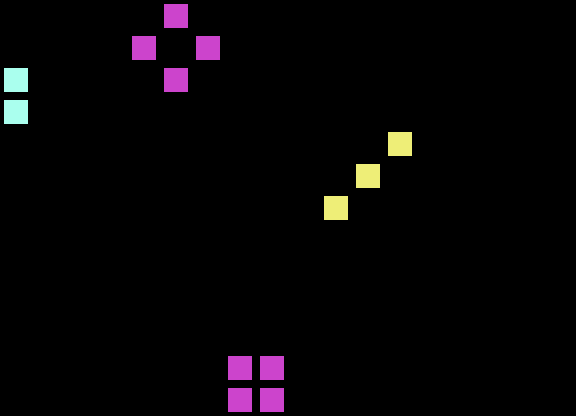
\includegraphics[width=1.3cm]{src/patterns/pixels/pixel_pattern14_6.png}%
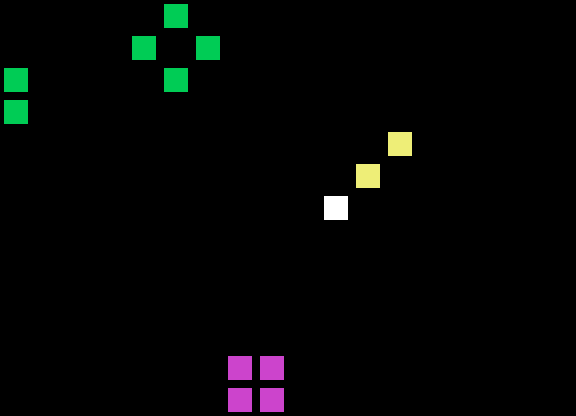
\includegraphics[width=1.3cm]{src/patterns/pixels/pixel_pattern14_7.png}%
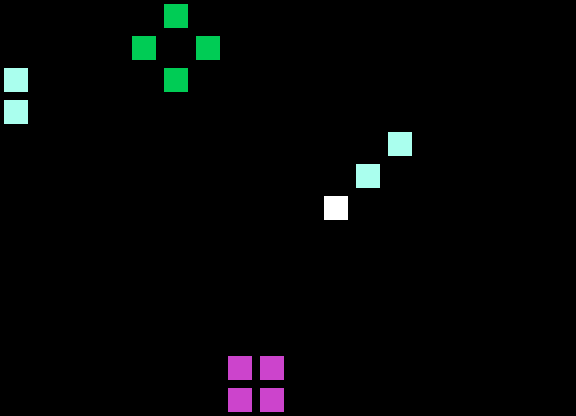
\includegraphics[width=1.3cm]{src/patterns/pixels/pixel_pattern14_8.png}%
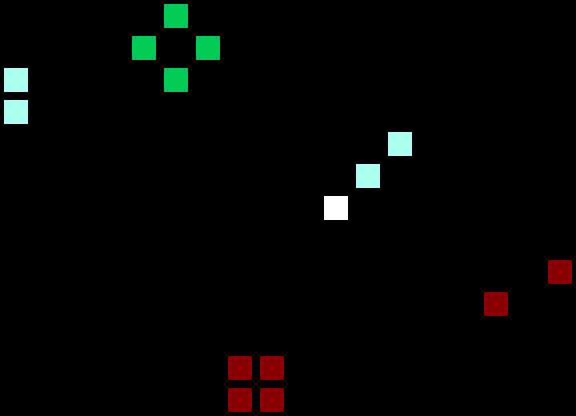
\includegraphics[width=1.3cm]{src/patterns/pixels/pixel_pattern14_9.png}%
} \\
        \midrule

        \makecell[l]{
\icode{.BYTE \$00,\$05,\$07}\\
\icode{.BYTE \$00,\$03,\$02}
} & \makecell[l]{
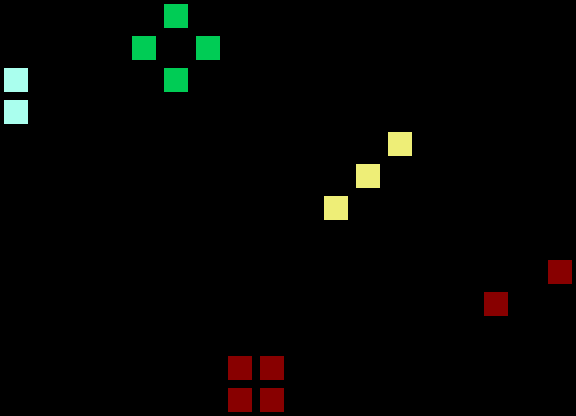
\includegraphics[width=1.3cm]{src/patterns/pixels/pixel_pattern14_10.png}%
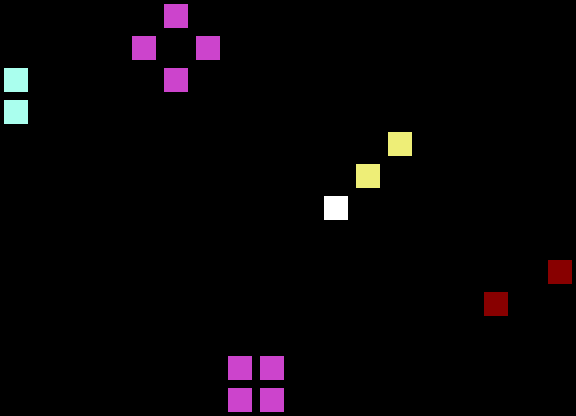
\includegraphics[width=1.3cm]{src/patterns/pixels/pixel_pattern14_11.png}%
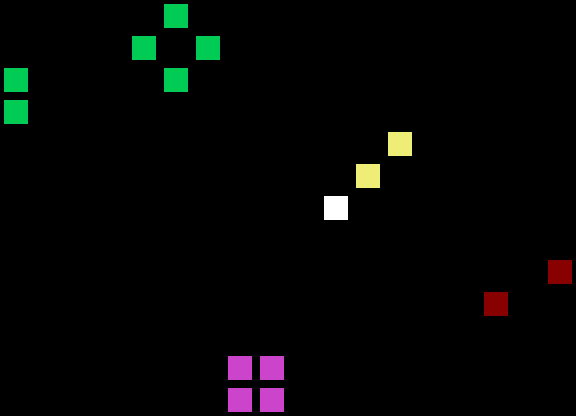
\includegraphics[width=1.3cm]{src/patterns/pixels/pixel_pattern14_12.png}%
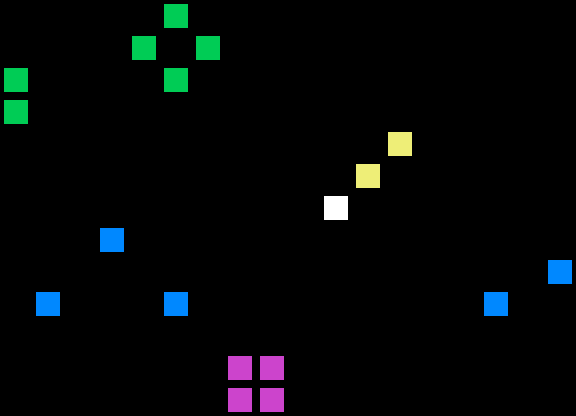
\includegraphics[width=1.3cm]{src/patterns/pixels/pixel_pattern14_13.png}%
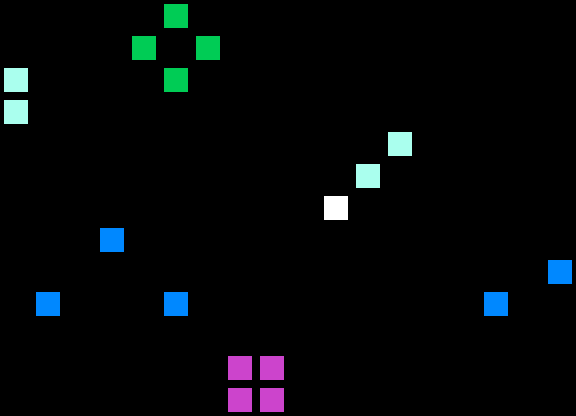
\includegraphics[width=1.3cm]{src/patterns/pixels/pixel_pattern14_14.png}%
} \\
        \midrule

        \makecell[l]{
\icode{.BYTE \$00,\$F9,\$F7,\$FB}\\
\icode{.BYTE \$00,\$01,\$03,\$03}
} & \makecell[l]{
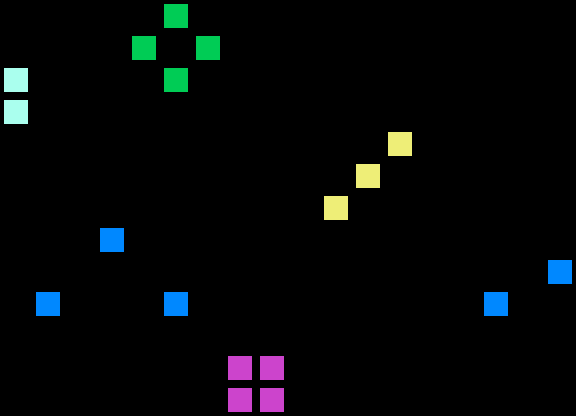
\includegraphics[width=1.3cm]{src/patterns/pixels/pixel_pattern14_15.png}%
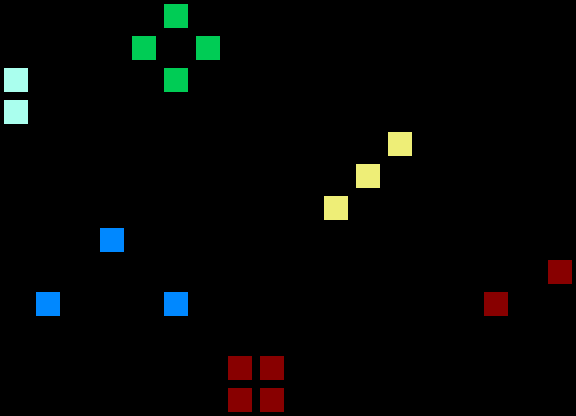
\includegraphics[width=1.3cm]{src/patterns/pixels/pixel_pattern14_16.png}%
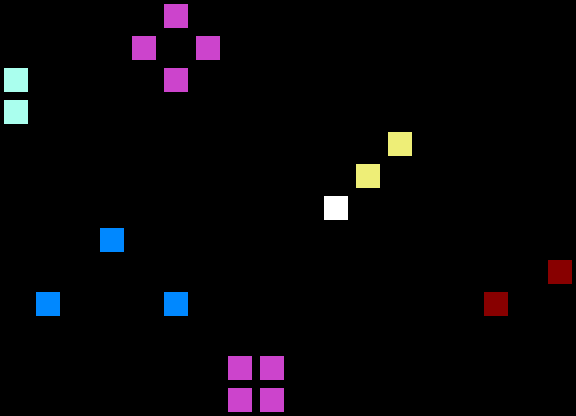
\includegraphics[width=1.3cm]{src/patterns/pixels/pixel_pattern14_17.png}%
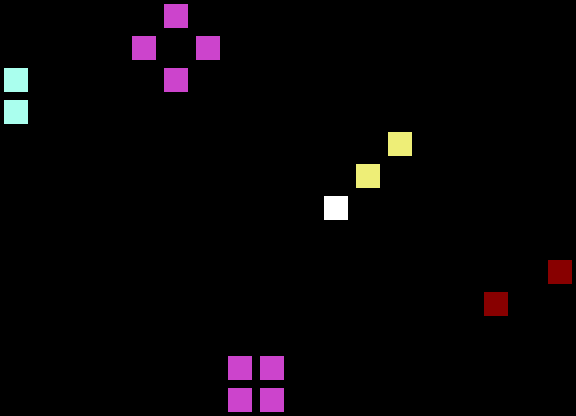
\includegraphics[width=1.3cm]{src/patterns/pixels/pixel_pattern14_18.png}%
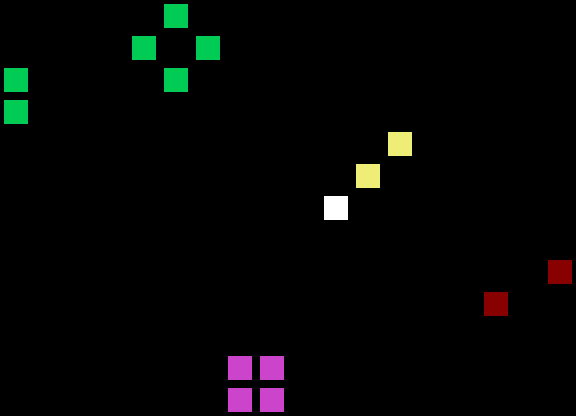
\includegraphics[width=1.3cm]{src/patterns/pixels/pixel_pattern14_19.png}%
} \\
        \midrule

        \makecell[l]{
\icode{.BYTE \$00}\\
\icode{.BYTE \$00}
} & \makecell[l]{
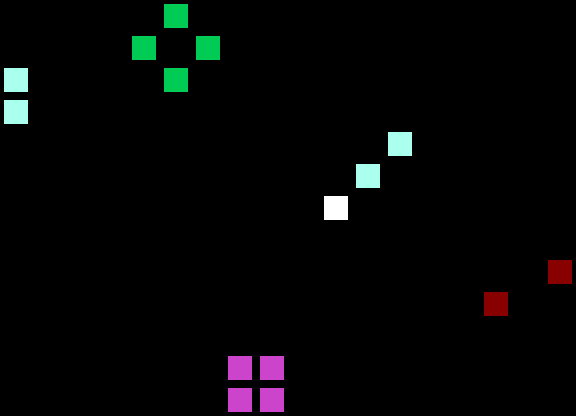
\includegraphics[width=1.3cm]{src/patterns/pixels/pixel_pattern14_20.png}%
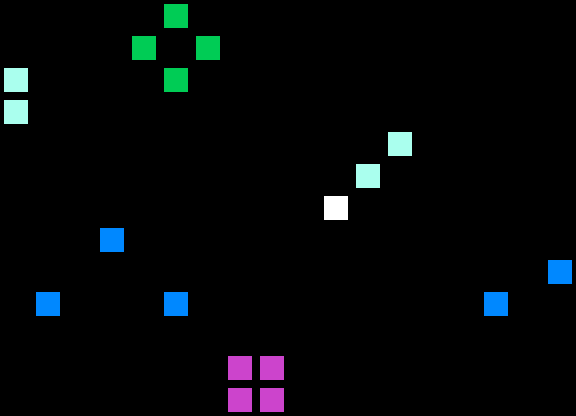
\includegraphics[width=1.3cm]{src/patterns/pixels/pixel_pattern14_21.png}%
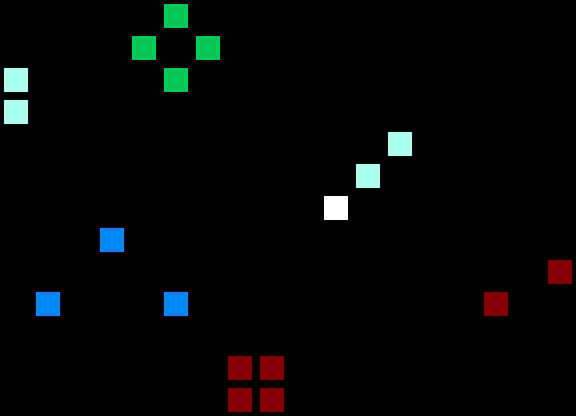
\includegraphics[width=1.3cm]{src/patterns/pixels/pixel_pattern14_22.png}%
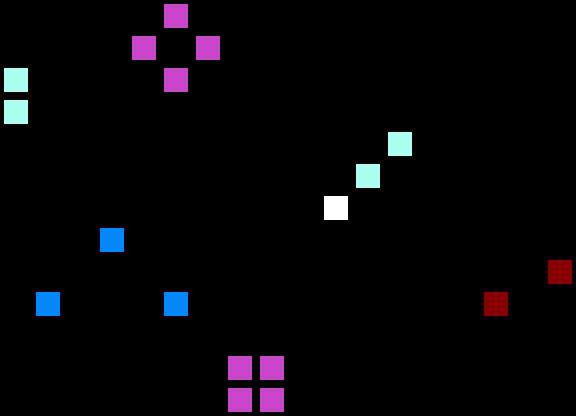
\includegraphics[width=1.3cm]{src/patterns/pixels/pixel_pattern14_23.png}%
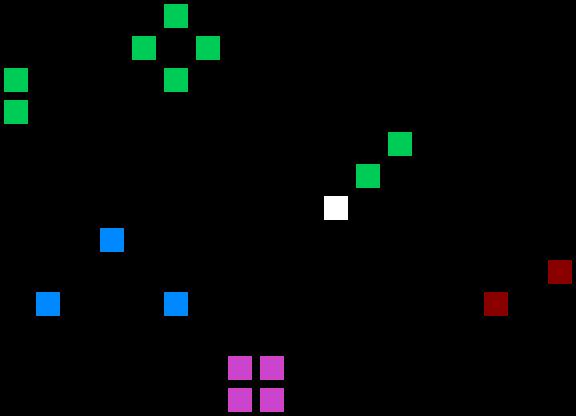
\includegraphics[width=1.3cm]{src/patterns/pixels/pixel_pattern14_24.png}%
} \\
        \midrule

        \makecell[l]{
\icode{.BYTE \$00}\\
\icode{.BYTE \$00}
} & \makecell[l]{
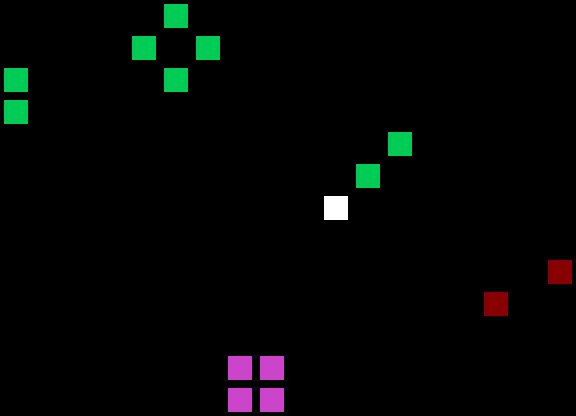
\includegraphics[width=1.3cm]{src/patterns/pixels/pixel_pattern14_25.png}%
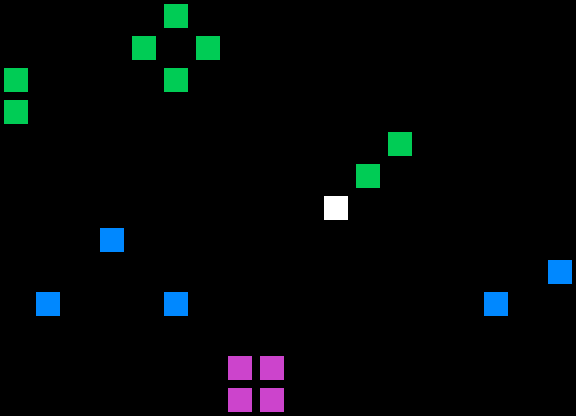
\includegraphics[width=1.3cm]{src/patterns/pixels/pixel_pattern14_26.png}%
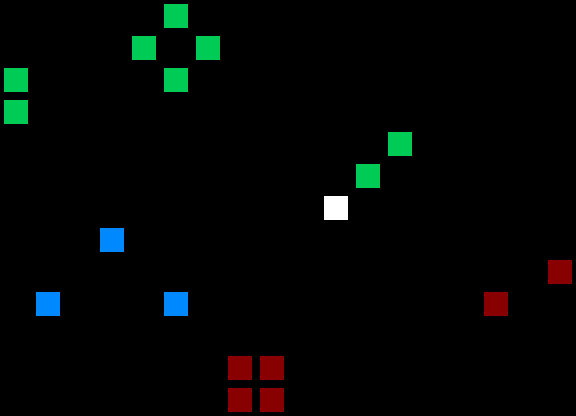
\includegraphics[width=1.3cm]{src/patterns/pixels/pixel_pattern14_27.png}%
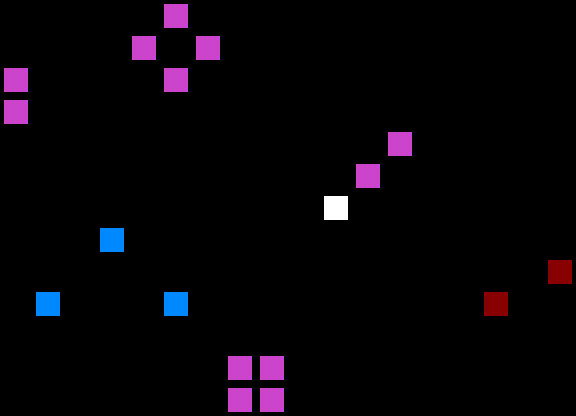
\includegraphics[width=1.3cm]{src/patterns/pixels/pixel_pattern14_28.png}%
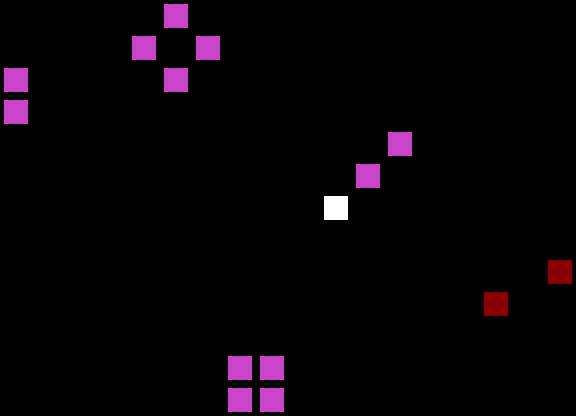
\includegraphics[width=1.3cm]{src/patterns/pixels/pixel_pattern14_29.png}%
} \\
        \midrule

      \end{tabular}
    \end{adjustbox}
  }\caption{The purpose of each of the oscillator values.}
\end{figure}
